
\documentclass{article}
\usepackage{graphicx} % Required for inserting images
\graphicspath{ {./images/} }
\usepackage{amsfonts}
\usepackage{mathtools}
\usepackage{mathrsfs}
\usepackage{amsmath}
\newcommand\aug{\fboxsep=-\fboxrule\!\!\!\fbox{\strut}\!\!\!}
\usepackage{tikz}
\usepackage{xfrac}
\usepackage{graphicx}

\title{Cullen Detecting NN}
\author{Sara Pessognelli}
\begin{document}
    \maketitle
    \section{Hamburgers Vs. Hotdogs}
    To begin this journey, we are going to start with an extremely basic classification problem: classifying hamburgers versus hotdogs based on 1) the amount of mustard
    and 2) the amoun of ketchup on each. We can then build on this framework to make more complex neural networks, like and MNIST handwritten digits classification NN, and finally
    a Cullen recognition NN. \\\\

    The first thing we'll talk about \textbf{Forward Propagation.} This is first step in the Neural Network's learning process.
    \section{Foward Propagation}
    Forward propagation basically amounts to the NN making a "guess" about the response, based on the given features. The NN will have various layers, the first of which is the 
    \textbf{input layer}, which takes the raw feature data for each obseravtion 
    \subsection{Neurons}
    \subsection{Activation Functions}
    \subsection{Cost Functions}
    \section{Back Propagation}
    \subsection{Gradient Descent}
    \section{Neural Network Architecture}
    We will build a network with 3 layers: an input layer, a ReLU layer, and finally the softmax layer. We will use cross-entropy for our cost (aka loss) function. There are reasons why we chose 
    this specific architecture, but we won't get into the weeds of it right now. Just know that these choices are best for this example. 
    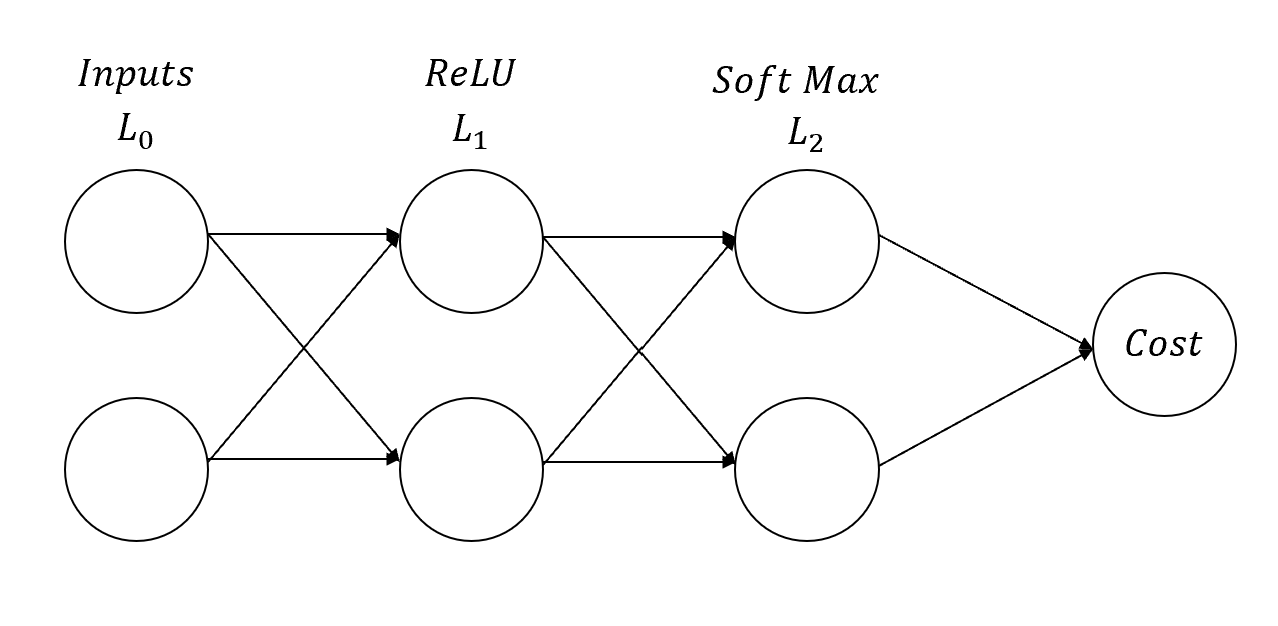
\includegraphics{architecture.png}\\\\
    Looking at the architecture above, let's tackle \textbf{Forward Propagation} first.
    \subsection{Forward Propagation.}
    Let's talk about our data and what it represents. This is some data that was made specifically for this proof of concept hamburger vs. hotdog NN:\\\\
    insert pic here \\\\
    some other stuff adibgdisbdisaubdiuasbdiubaiudsbfiudsbfuidsf
    siobfgifdsbgidfsbgiufdbgiudfsgbiusdfgbiudsfgbuidsfgbisudgbisudfgbuidfsgbfidusgbiudfsg
    sofdgnsdfgbaoiutuiertgweurtr9e8t\\\\
    We've chosen the cross-entropy cost function:
    $$C = Yln(A_2)+(1-Y)ln(1-A_2)$$
    We know for gradient descent we want to find $\frac{\partial C}{\partial A_2}$, which is
    $$\frac{\partial C}{\partial A_2} = \frac{-Y}{A_2} + \frac{1-Y}{1-A_2} = A_2(A_2-1)$$
    That's the easy part. Of course, we are going to need to find the partial derivatives for \textbf{all} our weights and biases. These will tell us how much
    impact each weight or bias has on the final $C$:
    \begin{thebibliography}{9}
        \bibitem{texbook}
        Donald E. Knuth (1986) \emph{The \TeX{} Book}, Addison-Wesley Professional.
        
        \bibitem{lamport94}
        Leslie Lamport (1994) \emph{\LaTeX: a document preparation system}, Addison
        Wesley, Massachusetts, 2nd ed.
        \end{thebibliography}
\end{document}